
\section{Data Processing}
\label{sec:data}

Data processing constructs samples from raw data recorded by Leap Motion, and consists of \textit{outlier elimination}, \textit{word segmentation}, and \textit{sample generation}. 



%%%
%%\begin{figure}[t]
%%%\small
%%\centering
%%\vspace{2mm}
%%\begin{tabular}{|c||c|c|c|c|c|c|}
%%\hline %\hline
%%Sample & \multicolumn{4}{c|}{s1}  & \multicolumn{2}{c|}{s2} \\ \hline
%%\# Frames  &231   &169   &231   &149   &260   &144      \\
%%User 1
%%&{
\includegraphics[width=0.07\columnwidth,totalheight=.018\textheight]{./Graphic/words_jing/1001_pdf.eps}}
%%&{
\includegraphics[width=0.07\columnwidth,totalheight=.018\textheight]{./Graphic/words_jing/1002_pdf.eps}}
%%&{
\includegraphics[width=0.07\columnwidth,totalheight=.018\textheight]{./Graphic/words_jing/1003_pdf.eps}}
%%&{
\includegraphics[width=0.07\columnwidth,totalheight=.018\textheight]{./Graphic/words_jing/1004_pdf.eps}}
%%&{
\includegraphics[width=0.07\columnwidth,totalheight=.018\textheight]{./Graphic/words_jing/1005_pdf.eps}}
%%&{
\includegraphics[width=0.07\columnwidth,totalheight=.018\textheight]{./Graphic/words_jing/1007_pdf.eps}}\\ \hline \hline
%%
%%Sample   &\multicolumn{2}{c|}{s1} &\multicolumn{2}{c|}{s2} &\multicolumn{2}{c|}{s3}  \\ \hline
%%\# Frames &466  & 288   &430   &183   &512   &264       \\
%%User 2
%%&{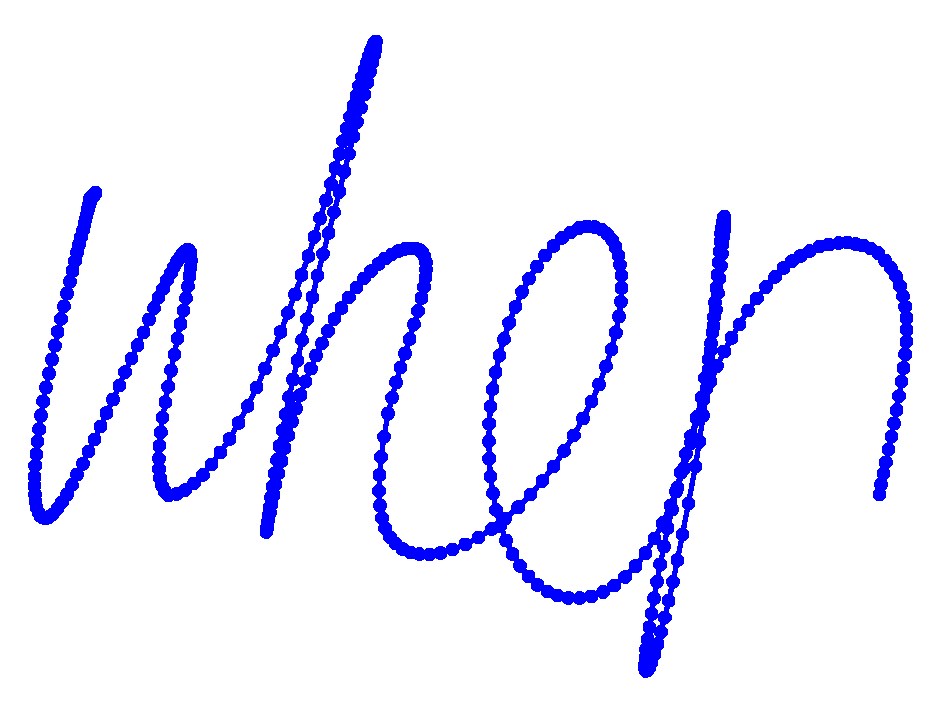
\includegraphics[width=0.07\columnwidth,totalheight=.018\textheight]{./Graphic/words_meng/10001_pdf.eps}}
%%&{
\includegraphics[width=0.07\columnwidth,totalheight=.018\textheight]{./Graphic/words_meng/10002_pdf.eps}}
%%&{
\includegraphics[width=0.07\columnwidth,totalheight=.018\textheight]{./Graphic/words_meng/10003_pdf.eps}}
%%&{
\includegraphics[width=0.07\columnwidth,totalheight=.018\textheight]{./Graphic/words_meng/10004_pdf.eps}}
%%&{
\includegraphics[width=0.07\columnwidth,totalheight=.018\textheight]{./Graphic/words_meng/10005_pdf.eps}}
%%&{
\includegraphics[width=0.07\columnwidth,totalheight=.018\textheight]{./Graphic/words_meng/10007_pdf.eps}}\\ \hline 
%%
%%\end{tabular}\vspace{-0mm}
%%\caption{An illustration of constructing samples from a group of words. { 
%%%The frame numbers and sample labels of each word segment are listed, and a
%%All the word segments with the same sample label (e.g., s1, s2) constitute a  sample. 
%%Given each sample length $L_s$ is no larger than 800 frames, $6$ words form different numbers of samples for Users 1 and 2.% , due to the different writing speeds.
%%} \vspace{0mm}}\label{fig:dataWords}
%%\end{figure}



\subsection{Leap Motion Data}
Leap Motion captures finger movements in a 3D space (as shown in \figref{fig:leap}):  the left-right motion will be recorded at the $x$-direction, the up-down motion at $y$-direction and the forward-backward motion at the $z$-direction. 
As a user raises his/her hands and uses one of the fingers to write,  a Leap Motion controller will capture information of up to 10 fingers (depending on their visibility). We extract the data of the foremost fingertip (i.e., the ones with the smallest $z$-value among all captured figures), and record a 11-dimensional vector with the information provided directly by Leap Motion (listed below) at time $t$ as a \textit{frame}.  
%\begin{inlinenum}
\begin{enumerate}
\setlength{\itemsep}{-0.5mm}
\item fingertip position,\quad -- $(p_x(t), p_y(t),p_z(t))$, 
\item fingertip velocity,\quad -- $(v_x(t), v_y(t),v_z(t))$, 
\item fingertip direction,\quad -- $(D_x(t), D_y(t),D_z(t))$, 
\item finger visible length and width.\quad -- $L_f(t)$ and $W_f(t)$. 
\end{enumerate}
%\end{inlinenum}
In addition, Leap Motion provides an ID number and a timestamp for each frame. The ID number of each frame for objects (e.g., fingers) is given as a positive number if at least one object is detected or becomes a negative number if no recognizable objects are detected. Thus, we utilize the ID numbers to check the validity of a frame and utilize timestamps to calculate the speed of handwriting. 
For each round of recording, Leap Motion will record a collection of  frames, by sequentially connecting all consecutive frames, we construct a raw handwriting trajectory.  



\begin{figure}[!t]
\vspace{-2mm}
\centering

\begin{tabular}{cc}
\subfigure[]
{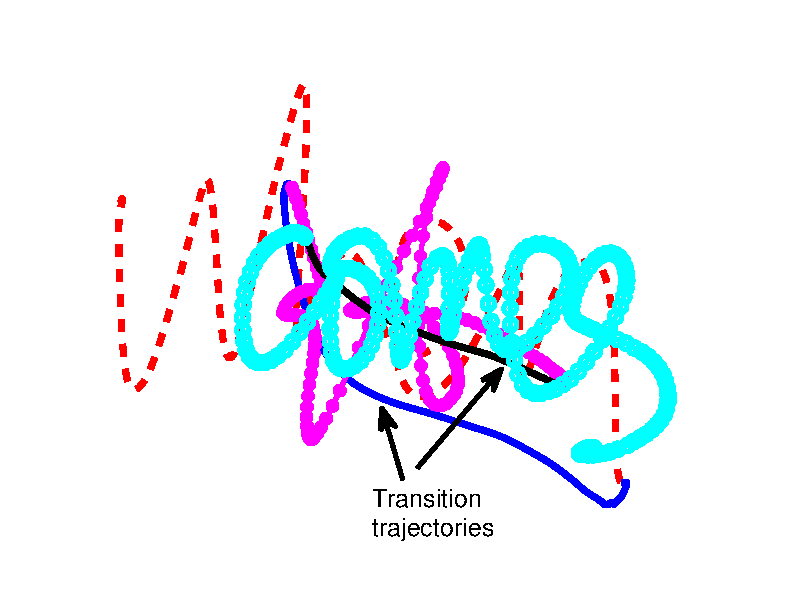
\includegraphics[width=0.45\columnwidth]{./Graphic/Pic_words_forSystemSection/segmentation1.pdf}} 
\subfigure[]
{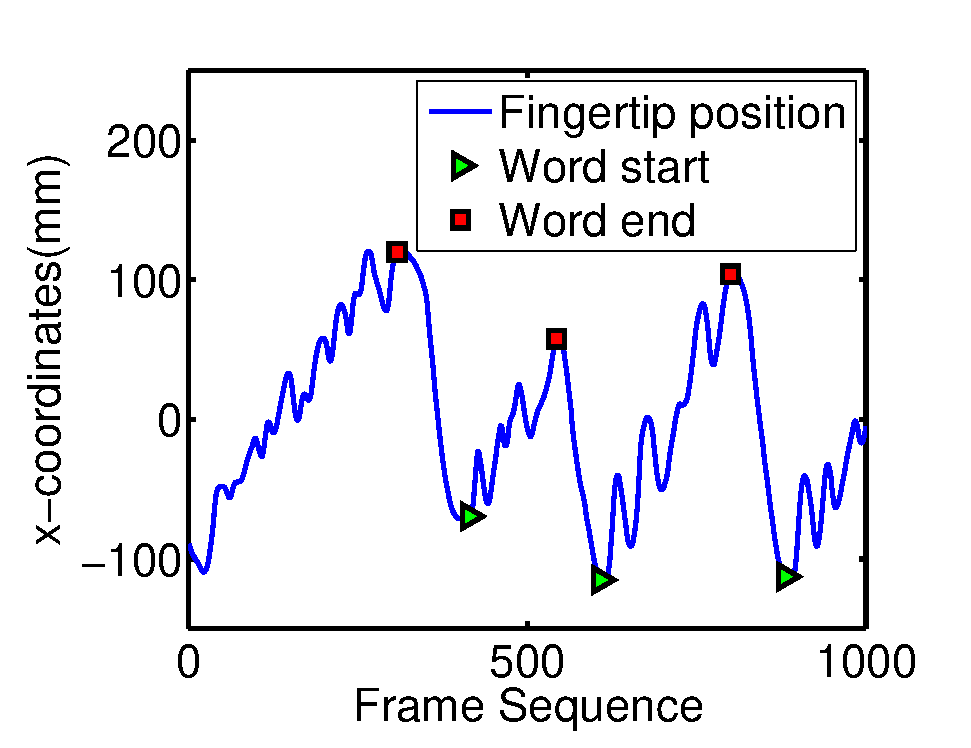
\includegraphics[width=.45\columnwidth]{./Graphic/pictures_seg/x-seg_1.eps}} 
%&\subfigure[]
%{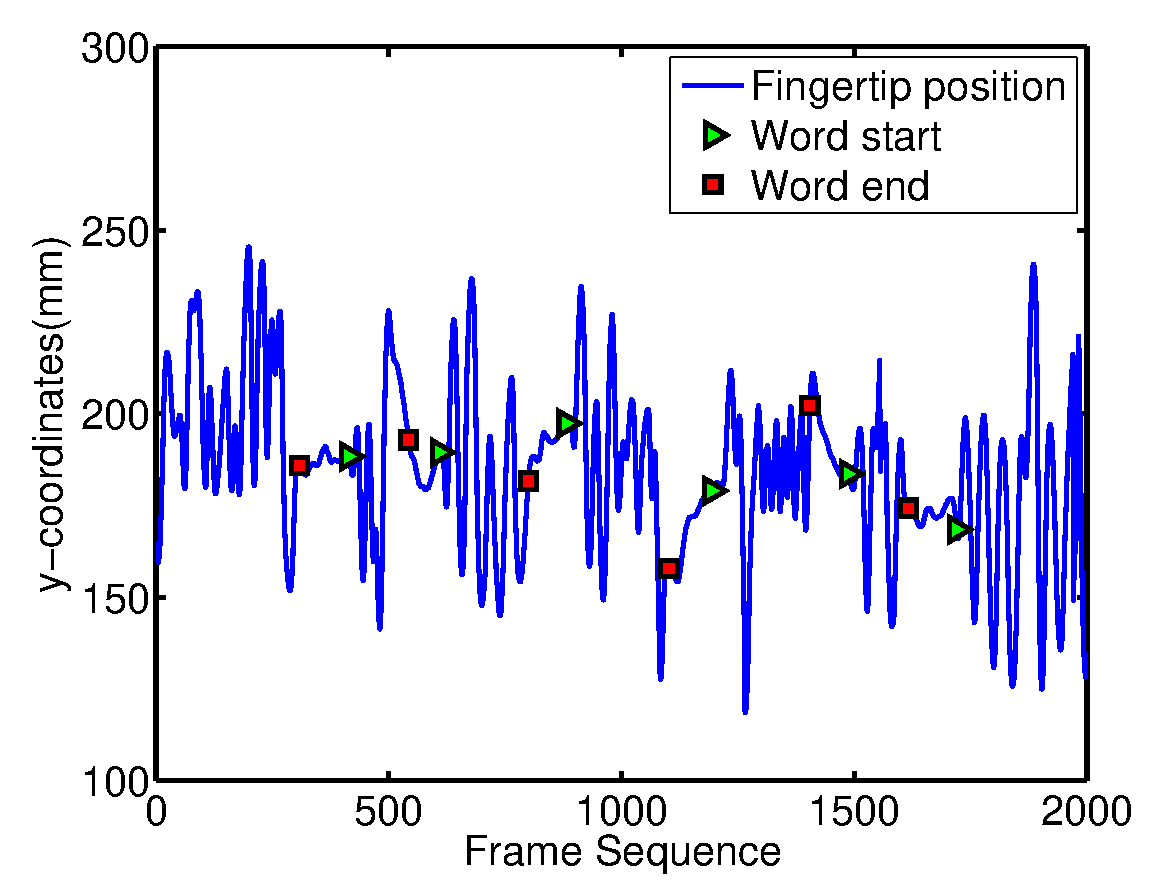
\includegraphics[width=.6\columnwidth]{./Graphic/pictures_seg/y-seg.eps}} 
%&\subfigure[]
%{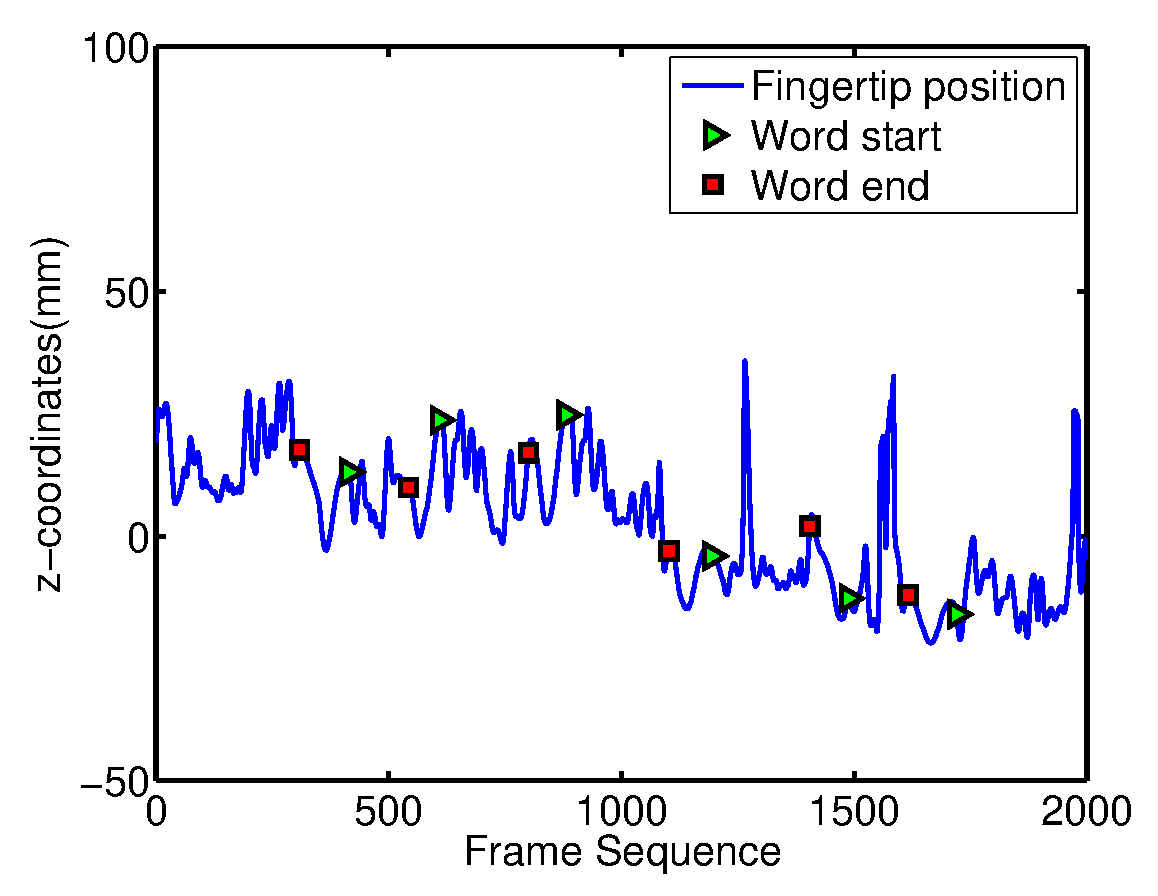
\includegraphics[width=.6\columnwidth]{./Graphic/pictures_seg/z-seg.eps}}
\end{tabular}
\begin{tabular}{ccc}

\begin{tabular}{c}
{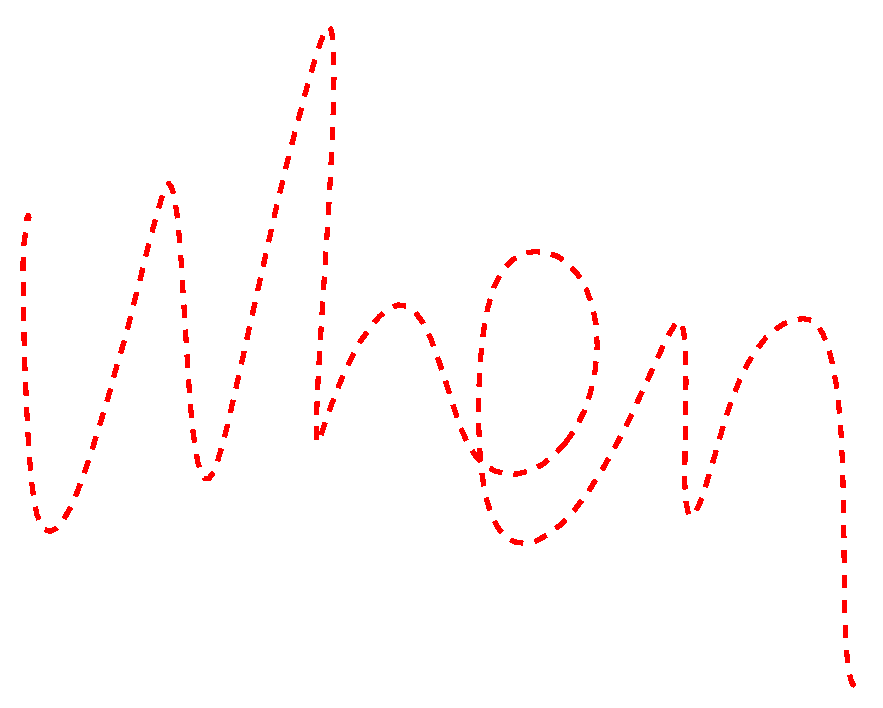
\includegraphics[width=0.22\columnwidth]{./Graphic/Pic_words_forSystemSection/1_thWord.eps}}
\end{tabular}
\vspace{-0mm}
& 
\begin{tabular}{c}
{
\includegraphics[width=0.22\columnwidth]{./Graphic/Pic_words_forSystemSection/2_thWord.eps}}
\end{tabular} 
\vspace{-0mm}
&
\begin{tabular}{c}
{
\includegraphics[width=0.22\columnwidth, height = 0.2\columnwidth]{./Graphic/Pic_words_forSystemSection/3_thWord.eps}} 
\end{tabular}
\vspace{-0mm} 
\\ 
\multicolumn{3}{c}{(c)} 

\end{tabular}

\vspace{-2mm}
\caption{{ {An illustration of word segmentation. (a) what was recorded by the Leap Motion controller, which contains three words and transition trajectories connecting them. (b) word segmentation results on x-axis. The trajectories starting from a red square and ending at the next green square are the transition ones, which are removed to obtain word segments. (c) shows the separated words from the trajectory in (a). \jingap{Note that the subject draw the point before the lower part of the letter `i'.}
}}\vspace{-0mm}}
\label{fig:segmentation}
\end{figure}




\begin{figure*}[ht]
\vspace{2mm}
\small
\centering
\begin{tabular*}{0.8\paperwidth}{ @{\extracolsep{\fill}} |p{0.9cm}|c||c|c|c|c|c|c|c|c|c|c|}
\hline %\hline
\multirow{12}{*}{User 1} 
& Sample Label & \multicolumn{9}{c|}{s1}  & s2 \\ \cline{2-12}
& \# Frames  &231   &169   &231   &149   &260   &144   &179   &305   &220   &356\\
& %User 1
&{
\includegraphics[width=0.07\columnwidth,totalheight=.018\textheight]{./Graphic/words_jing/1001_pdf.eps}}
&{
\includegraphics[width=0.07\columnwidth,totalheight=.018\textheight]{./Graphic/words_jing/1002_pdf.eps}}
&{
\includegraphics[width=0.07\columnwidth,totalheight=.018\textheight]{./Graphic/words_jing/1003_pdf.eps}}
&{
\includegraphics[width=0.07\columnwidth,totalheight=.018\textheight]{./Graphic/words_jing/1004_pdf.eps}}
&{
\includegraphics[width=0.07\columnwidth,totalheight=.018\textheight]{./Graphic/words_jing/1005_pdf.eps}}
&{
\includegraphics[width=0.07\columnwidth,totalheight=.018\textheight]{./Graphic/words_jing/1007_pdf.eps}}
&{
\includegraphics[width=0.07\columnwidth,totalheight=.018\textheight]{./Graphic/words_jing/1008_pdf.eps}}
&{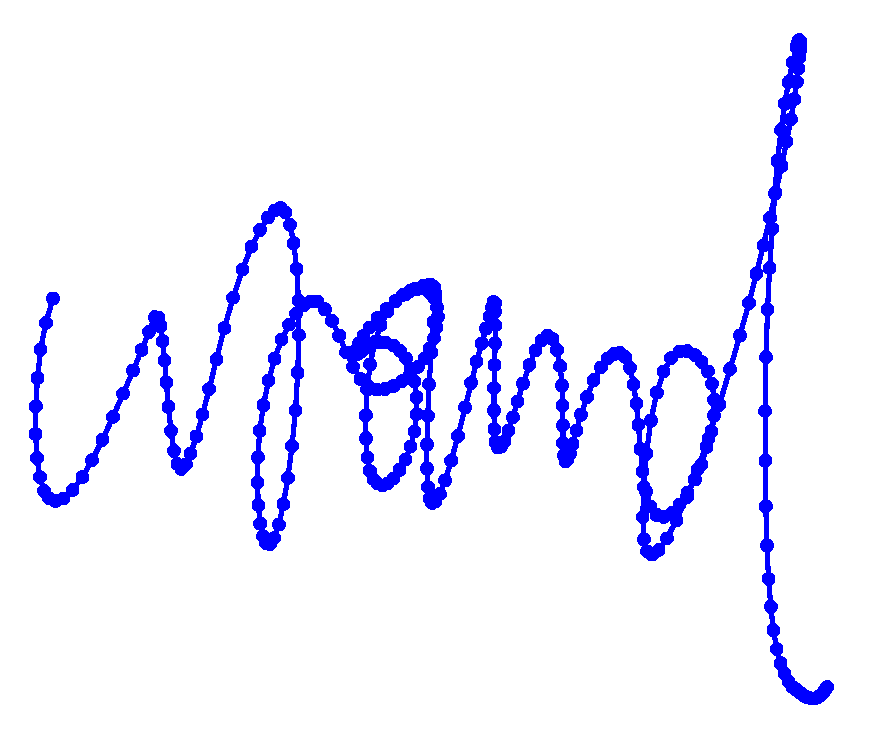
\includegraphics[width=0.08\columnwidth,totalheight=.018\textheight]{./Graphic/words_jing/1010_pdf.eps}}
&{
\includegraphics[width=0.08\columnwidth,totalheight=.018\textheight]{./Graphic/words_jing/1011_pdf.eps}}
&{
\includegraphics[width=0.08\columnwidth,totalheight=.018\textheight]{./Graphic/words_jing/1012_pdf.eps}}\\ 
& & \texttt{when}   &\texttt{it}   &\texttt{comes}  & \texttt{to} &\texttt{play}   &\texttt{do}   &\texttt{not}   &\texttt{would}   &\texttt{other}   & \texttt{speaks}  \\
\cline{2-12}
& Sample Label & \multicolumn{8}{c|}{s2}  & \multicolumn{2}{c|}{s3}   \\ \cline{2-12}
& \# Frames  &184   &214   &221  & 139  & 226    &98   &137   &210    &269  & 227 \\
& %User 1
&{
\includegraphics[width=0.07\columnwidth,totalheight=.018\textheight]{./Graphic/words_jing/1014_pdf.eps}}
&{
\includegraphics[width=0.07\columnwidth,totalheight=.018\textheight]{./Graphic/words_jing/1015_pdf.eps}}
&{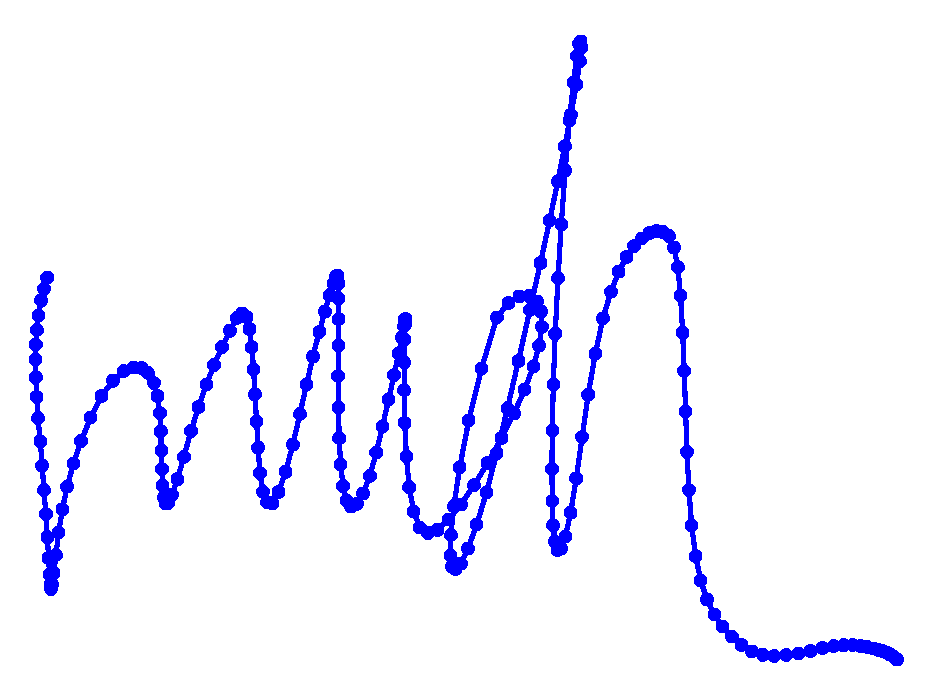
\includegraphics[width=0.07\columnwidth,totalheight=.018\textheight]{./Graphic/words_jing/1019_pdf.eps}}
&{
\includegraphics[width=0.07\columnwidth,totalheight=.018\textheight]{./Graphic/words_jing/1020_pdf.eps}}
&{
\includegraphics[width=0.08\columnwidth,totalheight=.018\textheight]{./Graphic/words_jing/1021_pdf.eps}}
&{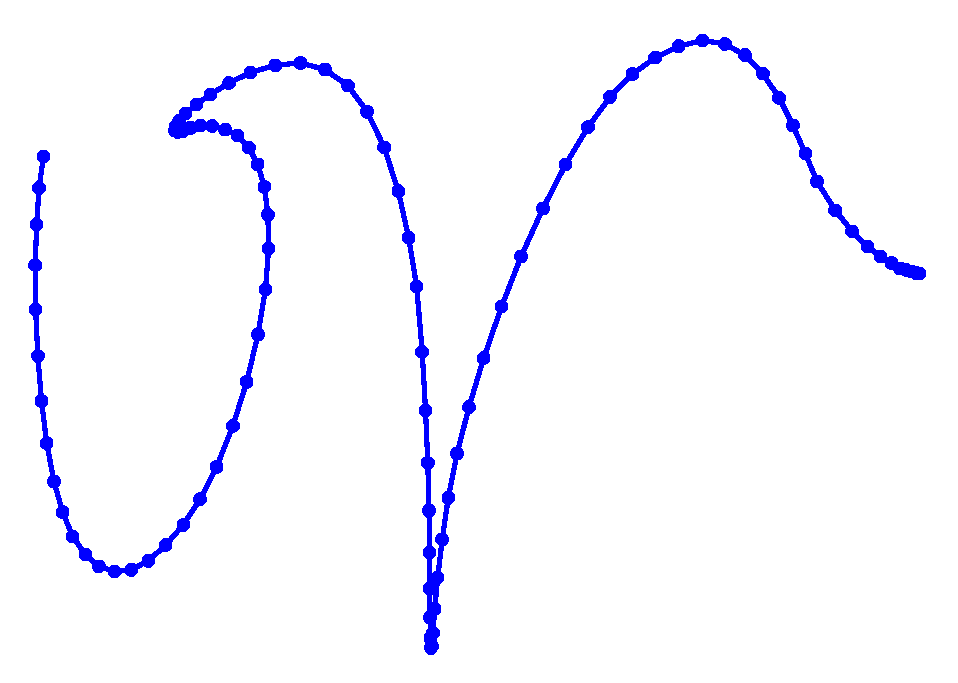
\includegraphics[width=0.07\columnwidth,totalheight=.018\textheight]{./Graphic/words_jing/1026_pdf.eps}}
&{
\includegraphics[width=0.07\columnwidth,totalheight=.018\textheight]{./Graphic/words_jing/1027_pdf.eps}}
&{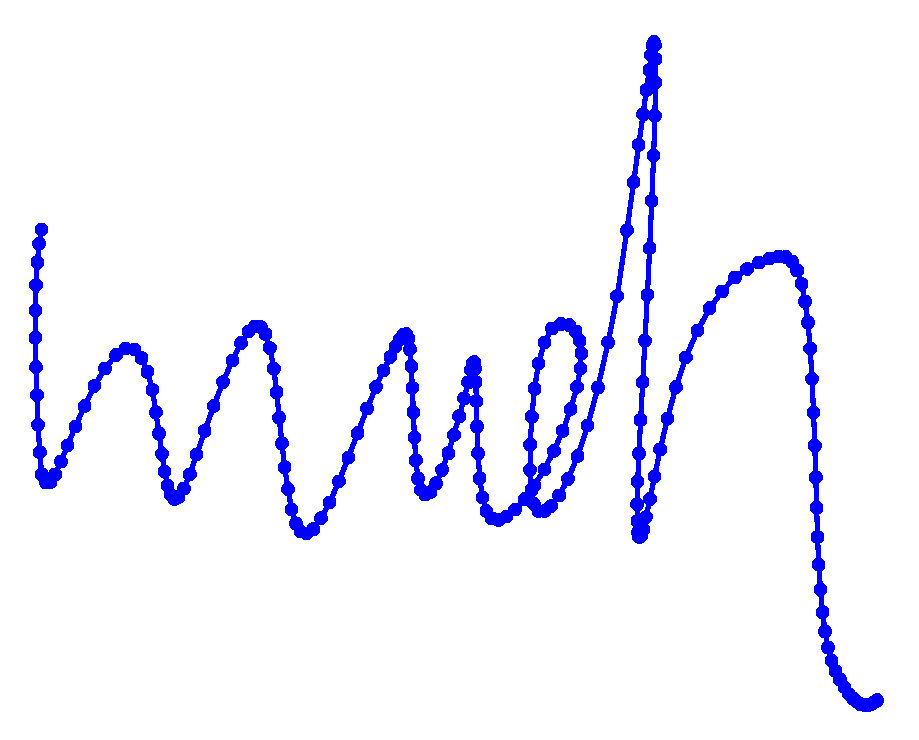
\includegraphics[width=0.07\columnwidth,totalheight=.018\textheight]{./Graphic/words_jing/1032_pdf.eps}}
&{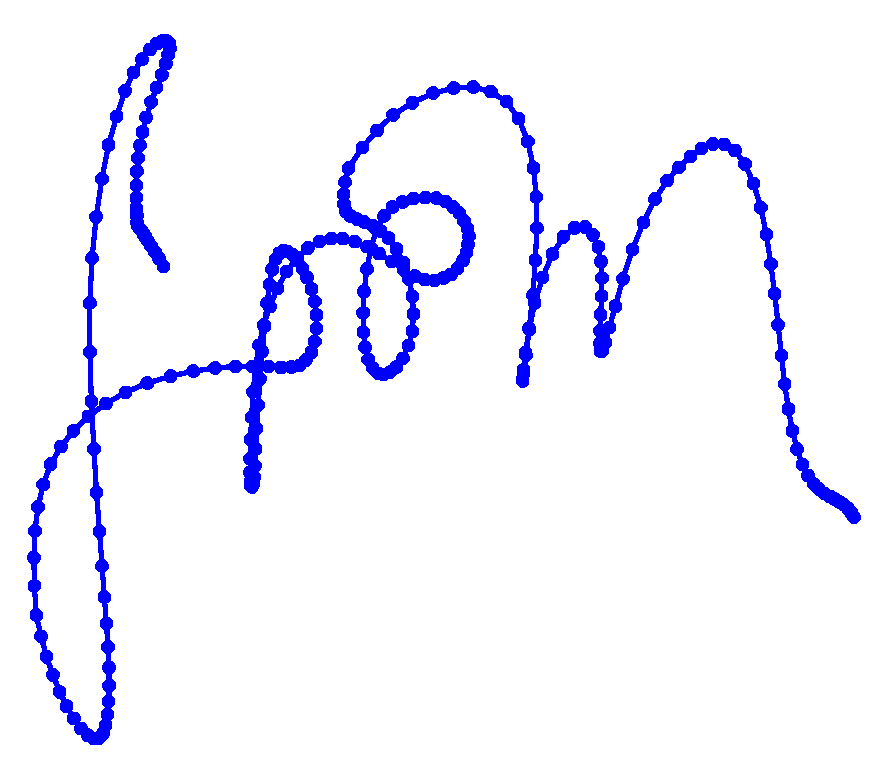
\includegraphics[width=0.07\columnwidth,totalheight=.018\textheight]{./Graphic/words_jing/1034_pdf.eps}}
&{
\includegraphics[width=0.07\columnwidth,totalheight=.018\textheight]{./Graphic/words_jing/4027_pdf.eps}}\\ 
& & \texttt{but}   &\texttt{note}   &\texttt{much}  & \texttt{of} &\texttt{their}   &\texttt{or}   &\texttt{as}   &\texttt{much}   &\texttt{from}   & \texttt{told}  \\
\cline{2-12}
& Sample Label & \multicolumn{7}{c|}{s3} & \multicolumn{3}{c|}{\textbf{s4}}  \\ \cline{2-12}
&\# Frames &136  &155  &238   &233  & 188 &  223  & 245  & 145   &191  & 178 \\
& %User 1
&{
\includegraphics[width=0.07\columnwidth,totalheight=.018\textheight]{./Graphic/words_jing/3011_pdf.eps}}
&{
\includegraphics[width=0.07\columnwidth,totalheight=.018\textheight]{./Graphic/words_jing/3016_pdf.eps}}
&{
\includegraphics[width=0.07\columnwidth,totalheight=.018\textheight]{./Graphic/words_jing/2003_pdf.eps}}
&{
\includegraphics[width=0.07\columnwidth,totalheight=.018\textheight]{./Graphic/words_jing/2008_pdf.eps}}
&{
\includegraphics[width=0.07\columnwidth,totalheight=.018\textheight]{./Graphic/words_jing/2014_pdf.eps}}
&{
\includegraphics[width=0.07\columnwidth,totalheight=.018\textheight]{./Graphic/words_jing/2015_pdf.eps}}
&{
\includegraphics[width=0.07\columnwidth,totalheight=.018\textheight]{./Graphic/words_jing/2018_pdf.eps}}
&{
\includegraphics[width=0.07\columnwidth,totalheight=.018\textheight]{./Graphic/words_jing/2016_pdf.eps}}
&{
\includegraphics[width=0.07\columnwidth,totalheight=.018\textheight]{./Graphic/words_jing/3001_pdf.eps}}
&{
\includegraphics[width=0.08\columnwidth,totalheight=.018\textheight]{./Graphic/words_jing/3002_pdf.eps}}\\ 
& & \texttt{one}   &\texttt{her}   &\texttt{game}  & \texttt{have} &\texttt{out}   &\texttt{what}   &\texttt{that}   &\texttt{it}   &\texttt{last}   & \texttt{summer}  \\
\hline 
\hline

\multirow{12}{*}{User 2} 
& Sample Label  &\multicolumn{5}{c|}{s1} &\multicolumn{4}{c|}{s2} &s3  \\ \cline{2-12}
& \# Frames &466  & 288   &430   &183   &512   &264  & 345  & 627   &499   &713  \\ 
& %User 2 
&{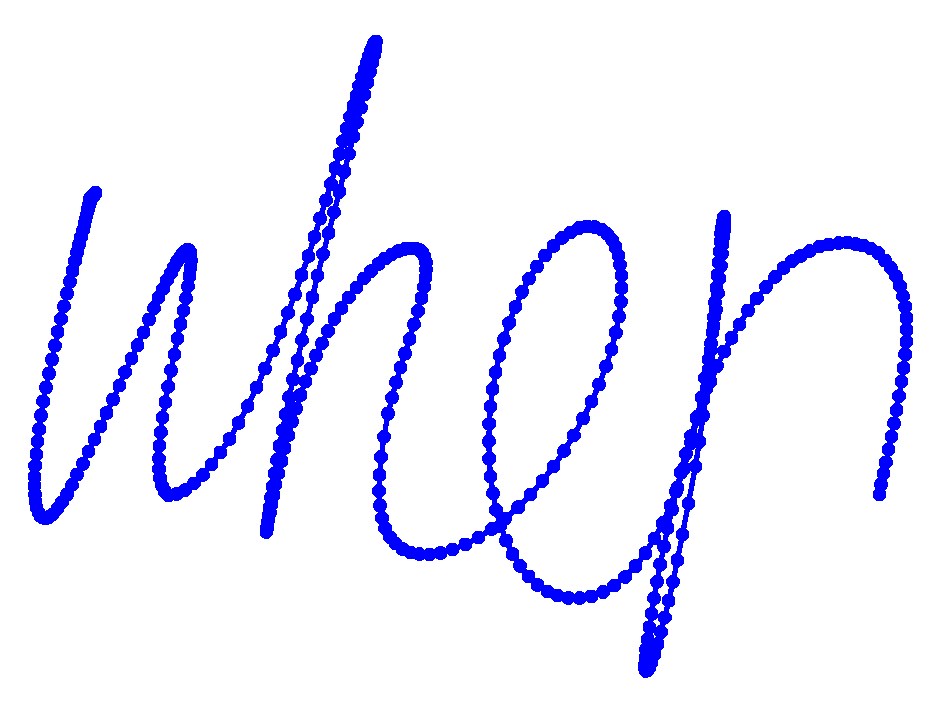
\includegraphics[width=0.07\columnwidth,totalheight=.018\textheight]{./Graphic/words_meng/10001_pdf.eps}}
&{\includegraphics[width=0.07\columnwidth,totalheight=.018\textheight]{./Graphic/words_meng/10002_pdf.eps}}
&{\includegraphics[width=0.07\columnwidth,totalheight=.018\textheight]{./Graphic/words_meng/10003_pdf.eps}}
&{\includegraphics[width=0.07\columnwidth,totalheight=.018\textheight]{./Graphic/words_meng/10004_pdf.eps}}
&{\includegraphics[width=0.07\columnwidth,totalheight=.018\textheight]{./Graphic/words_meng/10005_pdf.eps}}
&{\includegraphics[width=0.07\columnwidth,totalheight=.018\textheight]{./Graphic/words_meng/10007_pdf.eps}}
&{\includegraphics[width=0.07\columnwidth,totalheight=.018\textheight]{./Graphic/words_meng/10008_pdf.eps}}
&{\includegraphics[width=0.08\columnwidth,totalheight=.018\textheight]{./Graphic/words_meng/10010_pdf.eps}}
&{\includegraphics[width=0.08\columnwidth,totalheight=.018\textheight]{./Graphic/words_meng/10011_pdf.eps}}
&{\includegraphics[width=0.08\columnwidth,totalheight=.018\textheight]{./Graphic/words_meng/10012_pdf.eps}}\\ 
& & \texttt{when}   &\texttt{it}   &\texttt{comes}  & \texttt{to} &\texttt{play}   &\texttt{do}   &\texttt{not}   &\texttt{would}   &\texttt{other}   & \texttt{speaks}  \\
\cline{2-12} 
& Sample Label &\multicolumn{3}{c|}{s3} &\multicolumn{6}{c|}{s4} & s5  \\  \cline{2-12}
& \# Frames &364   &384  & 481  & 259 &  498  & 220  & 162   &399  & 454 & 264 \\
& %User 2
&{\includegraphics[width=0.07\columnwidth,totalheight=.018\textheight]{./Graphic/words_meng/10014_pdf.eps}}
&{\includegraphics[width=0.07\columnwidth,totalheight=.018\textheight]{./Graphic/words_meng/10015_pdf.eps}}
&{\includegraphics[width=0.07\columnwidth,totalheight=.018\textheight]{./Graphic/words_meng/10019_pdf.eps}}
&{\includegraphics[width=0.07\columnwidth,totalheight=.018\textheight]{./Graphic/words_meng/10020_pdf.eps}}
&{\includegraphics[width=0.08\columnwidth,totalheight=.018\textheight]{./Graphic/words_meng/10021_pdf.eps}}
&{\includegraphics[width=0.07\columnwidth,totalheight=.018\textheight]{./Graphic/words_meng/10026_pdf.eps}}
&{\includegraphics[width=0.07\columnwidth,totalheight=.018\textheight]{./Graphic/words_meng/10027_pdf.eps}}
&{\includegraphics[width=0.07\columnwidth,totalheight=.018\textheight]{./Graphic/words_meng/10032_pdf.eps}}
&{\includegraphics[width=0.07\columnwidth,totalheight=.018\textheight]{./Graphic/words_meng/10034_pdf.eps}}
&{\includegraphics[width=0.07\columnwidth,totalheight=.018\textheight]{./Graphic/words_meng/40027_pdf.eps}} \\ 
& & \texttt{but}   &\texttt{note}   &\texttt{much}  & \texttt{of} &\texttt{their}   &\texttt{or}   &\texttt{as}   &\texttt{much}   &\texttt{from}   & \texttt{told} \\
\cline{2-12}
& Sample Label &\multicolumn{5}{c|}{s5}  &\multicolumn{5}{c|}{\textbf{s6}}  \\  \cline{2-12}
& \# Frames  & 210 &217   &488   &381   &243   &352  & 399  & 211   &370   &251 \\
& %User 2
&{\includegraphics[width=0.07\columnwidth,totalheight=.018\textheight]{./Graphic/words_meng/30011_pdf.eps}}
&{\includegraphics[width=0.07\columnwidth,totalheight=.018\textheight]{./Graphic/words_meng/30016_pdf.eps}}
&{\includegraphics[width=0.07\columnwidth,totalheight=.018\textheight]{./Graphic/words_meng/20003_pdf.eps}}
&{\includegraphics[width=0.07\columnwidth,totalheight=.018\textheight]{./Graphic/words_meng/20008_pdf.eps}}
&{\includegraphics[width=0.07\columnwidth,totalheight=.018\textheight]{./Graphic/words_meng/20014_pdf.eps}}
&{\includegraphics[width=0.07\columnwidth,totalheight=.018\textheight]{./Graphic/words_meng/20015_pdf.eps}}
&{\includegraphics[width=0.07\columnwidth,totalheight=.018\textheight]{./Graphic/words_meng/20018_pdf.eps}}
&{\includegraphics[width=0.07\columnwidth,totalheight=.018\textheight]{./Graphic/words_meng/20016_pdf.eps}}
&{\includegraphics[width=0.07\columnwidth,totalheight=.018\textheight]{./Graphic/words_meng/30001_pdf.eps}}
&{\includegraphics[width=0.08\columnwidth,totalheight=.018\textheight]{./Graphic/words_meng/30002_pdf.eps}} \\
& & \texttt{one}   &\texttt{her}   &\texttt{game}  & \texttt{have} &\texttt{out}   &\texttt{what}   &\texttt{that}   &\texttt{it}   &\texttt{last}   & \texttt{summer} 
\\  
\hline 

%%\end{tabular*}\vspace{-0mm}
%%\caption{An illustration of constructing samples out of a group of words. 
%%Each word segment's frame numbers and sample labels are listed, and all the word segments with the same sample label constitute a  sample. For each user, $20$ word segments can construct different numbers of samples due to the different writing speeds.
%%The frame numbers and sample labels of each word segment are listed, and all the word segments with the same sample label (e.g., s1, s2) constitute a  sample. 
%%Given each sample length $L_s$ is no larger than 2000 frames, $20$ words form different numbers of samples for Users 1 and 2, due to the different writing speeds.
%%}\label{fig:dataWords}
%%\end{figure*}

\end{tabular*}\vspace{-0mm}
\caption{\jing{An illustration of constructing samples from a group of words.  
%The frame numbers and sample labels of each word segment are listed, and a
All the word segments with the same sample label (e.g., s1, s2) constitute a  sample. 
Given the sample length $L_s$ that is no larger than 2000 frames, $30$ words form around 4 or 6 samples for Users 1 and 2, respectively, due to the different writing speeds.
} \vspace{0mm}}\label{fig:dataWords}
\end{figure*}




\subsection{Outlier Elimination}
% define different noise types
Noises caused by environment variation may affect the Leap Motion raw trajectories. In general, such noises lead to abrupt changes of the fingertip positions between adjacent frames, as shown in Figure~\ref{fig:noises}. 
Therefore, they are actually outliers. In general, we observe two types of outliers: (1) no fingertip is detected ($7.32\%$ amount of data) , and (2) a fingertip is detected but at an unlikely position (less than $1\%$ amount of data). For no-detection cases, we examine the number of consecutive frames that do not contain detected fingertips. If the number is small, we perform spatial interpolation. If the number of noisy frames is large, we discard the noisy frames and divide the raw trajectory into two. 
Then we can perform the remaining data processing and feature extraction steps on each trajectory independently. 
For unlikely-position cases, we apply a temporal median filter to remove the outliers~\cite{SaltNoise}. 
At each frame, we examine a temporal window centered at this frame, search for the median of all values in this window,  and set the median as the new value of this frame. 
The median filter is applied not only on the $x$, $y$ and $z$ positions but also values on other dimensions. For both cases, our algorithm only removes the outliers and preserves the smoothness and continuity of the handwritings. 





%==================================================================



 \subsection{Word Segmentation}

The main goal of word segmentation is to identify the segments of the handwriting trajectories that contain useful information for recognizing handwriting styles. 
When writing on paper, we proceed from  left to right % and from the top to the bottom 
without text overwriting. % or connecting lines between words.
However, Leap Motion has limited writing space within which the hand motion can be captured -- after writing one or two words, a finger becomes out of the Leap Motion's field of view and it has to be moved back to the left.
As a result, finger trajectories of multiple words are overlapped and connected with transition trajectories that were traditionally invisible on paper, as shown in \figref{fig:segmentation} (a). %Thus, finger trajectories of real words shall be extracted, for displaying and analyzing.

%============================================== 

 
The transition trajectories shall be removed to extract real words. The key to identify such transition trajectories is to analyze the variations of $x$, $y$ and $z$-coordinates of
the handwriting trajectories (after the noise elimination). As a user writes from  left to right, the $x$-coordinates increases gradually. In comparison, re-positioning the hand back to the left bottom corner results in a sudden and large decrease of the $x$-value, as shown in Figure~\ref{fig:segmentation}(b), 
where the $x$-value periodically decreases since the user has to move the fingertip back to the left end frequently.
Thus, we identify transition trajectories by searching for a sequence of frames along which the $x$-value of fingertip positions monotonically decreases in a short period of time. By removing transition trajectories (e.g., starting from a red square and ending at the next green triangle as shown in~\ref{fig:segmentation}(b)), 
we obtain a set of disjoint word segments shown in~\ref{fig:segmentation}(c)). 
%The trajectories  are the transition ones, which are removed to obtain word segments. 
%\figref{fig:segmentation}(c) shows an example, where the overlapped handwriting trajectory depicted in \figref{fig:segmentation} (a) is divided into three separate word segments.

\jingap{\CiT sets hotkeys for starting a recording and stopping a recording. Before starting, finger(s) stay motionless and start writing after the press of the \texttt{start} hotkey. \CiT introduces a few data frames before the intent writing and includes these frames in the first word of a recording. The recording will be ended if any of the two scenarios happen: the finger(s) are out of the recording area or the \texttt{stop} hotkey is pressed. Thus, it is possible that extra frames are added to the last word before the recording ends completely.}



%==================================================================
\subsection{Sample Generation}
\label{subsec:sample}

The goal of sample generation is to create a set of samples. 
Since a single word may be too short to represent a user's handwriting style, we construct one sample with multiple word segments. %group of randomly selected word segments obtained in
%the word segmentation. 
We denote the total number of frames in a sample to be the \emph{length} of the sample. Ideally, the longer the sample length, the better the verification/identification performance. 
In practice, the length of samples should be small to ensure satisfying usability. In this paper, we conducted a series of experiments to understand the trade-off between usability and security, and determine the appropriate length of samples.

%\begin{figure}[t]
%\small
%\centering
%\begin{tabular}{|c||c|c|c|c|c|c|}
%\hline %\hline
%Sample & \multicolumn{4}{c|}{s1}  & \multicolumn{2}{c|}{s2} \\ \hline
%\# Frames  &231   &169   &231   &149   &260   &144      \\
%User 1
%&{\includegraphics[width=0.07\columnwidth,totalheight=.018\textheight]{./Graphic/words_jing/1001_pdf.eps}}
%&{\includegraphics[width=0.07\columnwidth,totalheight=.018\textheight]{./Graphic/words_jing/1002_pdf.eps}}
%&{\includegraphics[width=0.07\columnwidth,totalheight=.018\textheight]{./Graphic/words_jing/1003_pdf.eps}}
%&{\includegraphics[width=0.07\columnwidth,totalheight=.018\textheight]{./Graphic/words_jing/1004_pdf.eps}}
%&{\includegraphics[width=0.07\columnwidth,totalheight=.018\textheight]{./Graphic/words_jing/1005_pdf.eps}}
%&{\includegraphics[width=0.07\columnwidth,totalheight=.018\textheight]{./Graphic/words_jing/1007_pdf.eps}}\\ \hline \hline
%
%Sample   &\multicolumn{2}{c|}{s1} &\multicolumn{2}{c|}{s2} &\multicolumn{2}{c|}{s3}  \\ \hline
%\# Frames &466  & 288   &430   &183   &512   &264       \\
%User 2
%&{\includegraphics[width=0.07\columnwidth,totalheight=.018\textheight]{./Graphic/words_meng/10001_pdf.eps}}
%&{\includegraphics[width=0.07\columnwidth,totalheight=.018\textheight]{./Graphic/words_meng/10002_pdf.eps}}
%&{\includegraphics[width=0.07\columnwidth,totalheight=.018\textheight]{./Graphic/words_meng/10003_pdf.eps}}
%&{\includegraphics[width=0.07\columnwidth,totalheight=.018\textheight]{./Graphic/words_meng/10004_pdf.eps}}
%&{\includegraphics[width=0.07\columnwidth,totalheight=.018\textheight]{./Graphic/words_meng/10005_pdf.eps}}
%&{\includegraphics[width=0.07\columnwidth,totalheight=.018\textheight]{./Graphic/words_meng/10007_pdf.eps}}\\ \hline 
%
%\end{tabular}\vspace{-1mm}
%\caption{An illustration of constructing samples out of a group of words. { 
%The frame numbers and sample labels of each word segment are listed, and all the word segments with the same sample label (e.g., s1, s2) constitute a  sample. 
%Given each sample length $L_s$ is no larger than 800 frames, $6$ words form different numbers of samples for Users 1 and 2, due to the different writing speeds.} \vspace{-3mm}}\label{fig:dataWords}
%\end{figure}



Since various users may write at different speeds, the number of frames in each word segment of various users may differ. To avoid the impact of writing speeds, we construct a sample based on the frame length instead of the number of words. Figure~\ref{fig:dataWords} demonstrates an example.
%, where the top row lists $6$ word segments and the corresponding frame numbers from user 1, and the bottom row lists $6$ word segments from user 2. 
In this example, we construct samples with a sample length no greater than $2000$ frames. 
We concatenate as many word segments as possible into a sample until one extra segment will make the sample contain more than $2000$ frames. 
With $30$ word segments, user 1 can only create less than $4$ samples, and user 2 can create almost $6$ samples. % (sample IDs are listed on top of the frame number in each row).  This is because the average number of words in a sample is about four for user 1 and two for the user 2. 


%In section~\ref{sec:results}, we will conduct experiments to determine the appropriate sample length.

